\section{Scheduling}
E' l' attività di scegliere quale processo mandare in esecuzione e quale processo caricare in memoria centrale.

\subsection{Tipo di scheduling}
Si compone di 3 unità diverse:
\begin{figure}[H]
    \centering
    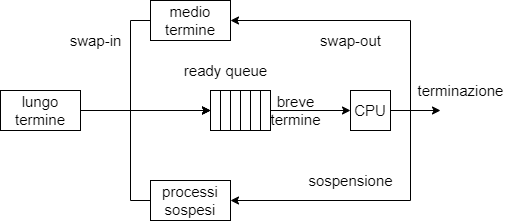
\includegraphics[width=300px]{images/4_Scheduling/scheduling.png}
\end{figure}

\subsubsection{A breve termine}
Sceglie quale processo, tra quelli pronti, mettere in esecuzione.
Interviene quando la CPU rimane libera per qualche motivo.
Può sia essere preemptive che non preemptive.

\subsubsection{A medio termine}
Si occupa di scegliere quale processo trasferire temporaneamente in memoria secondaria.
Questo è indispensabile nelle macchine in cui la memoria centrale non basta per accogliere tutti i processi in esecuzione.
E' anche detto \emph{swapping} perché richiede l' uso della paginazione su domanda, appunto, lo swap.

\subsubsection{A lungo termine}
Sceglie quale processo caricare dalla memoria secondaria alla memoria centrale.
Controlla quindi il grado di multiprogrammazione, cioè il numero di processi in memoria centrale e si occupa di scegliere una pool di processi eterogenea in termini di CPU bound e I/O bound.

E' una componente di minore importanza all' interno delle macchine general purpose comuni, tant' è che a volte non è neanche implementata.

\subsection{Metriche di valutazione}
Utiliziamo delle metriche per valutare i vari algoritmi che vedremo:
\begin{itemize}
    \item utilizzo della CPU
    \item tempo medio di completamento (\emph{turnaround time})
    \item produttività (\emph{throughput rate}): numero di processi terminati nell' unità di tempo
    (è l' inverso del turnaround)
    \item tempo di risposta: tempo necessario per terminare una volta partito (è il turnaround del singolo processo)
    \item tempo di attesa: somma degli intervalli di tempo nei quali il processo è in coda pronti
    \item rispetto dei vincoli temporali: utile nei sistemi operativi in tempo reale
\end{itemize}

\subsection{Algoritmi di scheduling}
Ci sono vari algoritmi per scegliere quale processo lanciare, vediamone alcuni.

\subsubsection{FCFS - First Come First Served}
Si crea una coda e si segue l'ordine con il quale sono arrivati i processi per metterli in esecuzione. Non preemptive.

In questo algoritmo non serve sapere la durata dei CPU burst (il tempo in cui il processo ha bisogno della CPU).
Può portare a lunghi tempi di attesa in quanto se un processo arriva tardi prima di essere messo in esecuzione bisogna che finiscano tutti quelli prima di lui.

\subsubsection{SJF - Shortest Job First}
Vedo nei descrittori la lunghezza (vera o stimata) del job e metto in esecuzione quello con il valore minore.

E' un primo algoritmo a priorità ma la priorità è statica ed è difficile dare una stima corretta!
Non preemptive. Questo algoritmo può portare alla \emph{starvation} dei processi più lunghi qualora ne arrivassero tanti di breve durata.
Per risolvere la starvation possiamo introdurre algoritmi di \emph{ageing}, cioè: più il processo rimane in coda e più la sua priorità aumenta, in questo modo anche quei processi lunghi che sono alla fine della lista di priorità verranno serviti con certezza.
Si noti tuttavia che algoritmi del genere possono aumentare l' overhead generale, ne va pertanto limitato l' utilizzo.

Può diminuire il turnaround medio ma anche il tempo medio di attesa proprio perché mette in esecuzione i processi più corti prima.

\subsubsection{SRTF - Shortest Remaining Time First}
Si mette in esecuzione il processo con tempo rimanente alla fine minore tra tutti. E' come il SJF ma ha una priorità dinamica in quanto il valore del tempo rimanente diminuisce ogni volta che il processo viene stoppato.
Ha un overhead maggiore dovuto a questo calcolo.
E' preemptive.

L'algoritmo parte ogni qual volta un processo va in coda pronti, si controlla se il nuovo processo ha priorità maggiore ed eventualmente si esegue la preemption.

Conoscere il CPU burst di un processo è fondamentale per questo algoritmo e per quello precedente, per macchine special purpose potrebbe essere semplice stimare il tempo dell' algoritmo sui dati in ingresso, sulle macchine general purpose che quindi possono eseguire molti algoritmi diversi la situazione è più complessa.
Si esegue quindi una stima del CPU burst utilizzando la media esponenziale che tiene conto della storia dei valori di durata dei CPU burst. Presi i vari $t_n$: durata effettiva del CPU burst ennesimo, $s_n$: la sua stima, $0 \leq a \leq 1$: un fattore a scelta, usiamo:
$$ s_{n+1} = at_n + (1-a)s_n $$

Si noti che usando $a = 0$ si ha che tutte le stime sono uguali alla stima iniziale, usando $a = 1$ invece non si tiene minimamente conto dello storico delle stime ma si usano solo i valori effettivamente misurati.
Tipicamente si usa $a = \frac{1}{2}$.
Nella pratica la nuova stima è composta da una certa percentuale della stima precedente e per la restante parte dal vero valore del CPU burst precedente.

\subsubsection{RR - Round Robin}    
Tipico algoritmo dei sistemi a time-sharing, si usa una coda come in FCFS ma al termine del quanto di tempo il processo si stoppa e si mette in esecuzione il prossimo, il corrente viene messo alla fine della coda.
In un certo senso è deterministico in quanto per sapere quando un processo verrà messo in esecuzione mi basta contare quanti processi ci sono in coda prima di lui e moltiplicarli per la durata del quanto di tempo.
E' molto comodo per quei sistemi con molti processi interattivi cioè processi con piccoli CPU burst ma grandi I/O burst come click del mouse, input da tastiera, ecc.

Segue sempre l'ordine di arrivo dei processi, è ovviamente preemptive e la revoca avviene sempre alla fine del quanto di tempo.

Le scelte da compiere nell'applicazione di questo algoritmo sono quelle relative alla durata del quanto di tempo, se lo faccio troppo piccolo infatti potrei frammentare troppo i processi ed avere un enorme overhead inutile, se lo faccio troppo grande potrebbe esserci poca responsività dei processi.
Con la giusta tempistica i processi piccoli terminano con poche interruzioni mentre i processi più lunghi sono spalmati su più tempo.

\subsubsection{Scheduling a code multiple}
I sistemi moderni non usano un singolo algoritmo ma più spesso un insieme di algoritmi in base alle necessità.
Possiamo pensare ad un sistema con più code pronti, ognuna delle quali con un algoritmo specifico, diamo i nomi alle code in base alla priorità associata:
\begin{figure}[H]
    \centering
    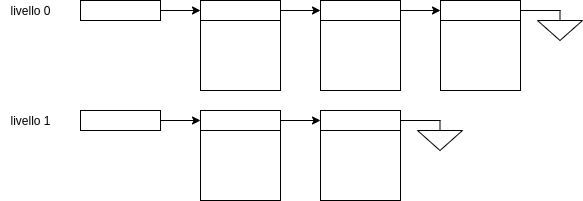
\includegraphics[width=300px]{images/4_Scheduling/code_multiple.png}
\end{figure}
decidiamo di gestire la coda di livello 0 tramite un round-robin e vi inseriamo all' interno quei processi con alta interazione, li eseguiamo finché possiamo, quando la coda si svuota passiamo alla coda di livello 1.
Se le code di livello inferiore sono sempre piene può esserci il problema della starvation da risolvere sempre con meccanismi di ageing.

Supponiamo che il livello 0 sia vuoto e che il livello 1 sia organizzato tramite FCFS, se partisse un processo dal livello 1 reintrodurrei la non preemption nel mio sistema, potrebbe essere un problema. Per risolvere questa situazione quando in esecuzione c'è un processo di livello 1 ed un processo entra in coda al livello 0 stoppo il processo corrente, lo inserisco nella testa della coda di livello 1 e metto in esecuzione il processo dal livello 0.

Questo algoritmo è molto utile nei sistemi IoT in quanto uso la coda di livello 0 per rispondere velocemente agli impulsi mentre uso la coda di livello 1 per eseguire calcoli. Nella pratica ho una gestione dei processi in foreground ed una gestione dei processi in background.

\subsubsection{Multi-level Feedback Queue}
Quando si ha a che fare con più code di processi si deve scegliere in qualche modo dove inserire i nuovi processi che arrivano.
Se riusciamo a sapere in qualche modo che tipo di processo è possiamo usare una banale tecnica:
\begin{itemize}
    \item I/O bound $\xrightarrow{}$ livello 0
    \item CPU bound $\xrightarrow{}$ livello 1
\end{itemize}
Se invece non abbiamo modo di saperlo in anticipo possiamo usare delle code con feedback.
Costruiamo 3 code:
\begin{itemize}
    \item livello 0: round robin con slot di 10ms
    \item livello 1: round robin con slot di 50ms
    \item livello 2: FCFS
\end{itemize}
\begin{figure}[H]
    \centering
    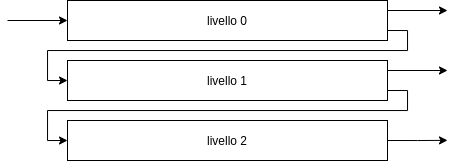
\includegraphics[width=300px]{images/4_Scheduling/feedback_queue.png}
\end{figure}
Quando un processo viene spawnato lo inserisco nella coda di livello 0, si applica la priorità tra le code, quindi finché ho elementi in coda 0 non tocco né coda 1 né coda 2, finché ho elementi in coda 1 non tocco la coda 2, e così via se avessi ancora più code.
Se la coda 0 è non vuota prendo un processo e lo metto in esecuzione, se termina ottimo, se non termina lo sposto alla fine della coda di livello 1.
Se la coda di livello 0 è vuota metto in esecuzione un processo dalla coda di livello 1, se termina bene, se non termina lo sposto alla fine della coda di livello 2.
Se sia la coda 0 che la coda 1 sono vuote metto in esecuzione un processo dalla coda 2.

Essendoci una priorità tra le code se è in esecuzione un processo da una coda più bassa ed in una coda pronti di priorità più alta viene aggiunto un nuovo processo si esegue preemption!
Inoltre per prevenire la starvation dei processi delle code con bassa priorità è necessario implementare meccanismi di aging che facciano saltare i processi verso code di priorità maggiore.

\subsection{Schedulazione di sistemi in tempo reale}
Si parla sempre di processi ma questa volta sono periodici.
Questi sistemi operativi si trovano all' interno di microcontrollori e devono gestire processi del tipo: read-eval-write.
Tempo reale perché il sistema deve essere in grado di evolvere avendo percezione del vero tempo che scorre in quanto deve avere coscienza degli intervalli di tempo.
Il criterio per il quale si lavora è \emph{garantire che il sistema faccia rispettare a tutti i processi le loro deadline}, questo perché se il processo farà tardi non sarà pronto a recepire il nuovo dato ed elaborarlo.
Questa condizione è detta di \emph{overflow}, se il sistema è \emph{hard real-time} questa condizione rende il sistema \emph{non schedulabile} e quindi non funzionerà, se il sistema è \emph{soft real-time} invece l' overflow è ammesso perché compromette solo la qualità del servizio, non la disponibilità.

\subsubsection{Ciclo di vita di un processo real time}
\begin{figure}[H]
    \centering
    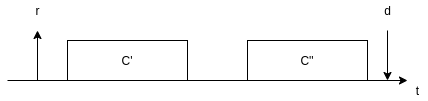
\includegraphics[width=300px]{images/4_Scheduling/processo_real_time.png}
\end{figure}
Possiamo distinguere i seguenti momenti:
\begin{itemize}
    \item $r$ - request: il processo entra in coda pronti
    \item $d$ - deadline: entro questo istante il processo deve aver terminato
    \item $C = C' + C''$: tempo di CPU necessario al completamento della computazione, in pratica il CPU burst
\end{itemize}
Si noti che ammettiamo uno scheduling preemptive in quanto il processo stesso è stato diviso in due burst $C'$ e $C''$.

\subsubsection{Generalizzazione dei processi}
Non sempre $C$ è conosciuto, per questo motivo bisogna saper valutare $C_{max}$, questo si può fare perché l' algoritmo eseguito dal processo è noto così come il range dei dati in ingresso!

Oltre alla stima della durata del task conosciamo anche la deadline $d$ ed il periodo $t$.
Supponiamo quindi di avere un processo $P_i$ che abbia durata stimata $C_i$, periodo $t_i$ ed ultima richiesta all' istante $r_k$, possiamo quindi dire:
$$ r_{k+1} = r_k + t_i $$
Sappiamo inoltre che $d_i \leq t_i$ in quanto altrimenti il problema sarebbe direttamente non schedulabile, approssimiamo quindi:
$$ r_{k+1} = r_k + t_i = d_k $$
Supponiamo che il prossimo istante nel quale si riceve la nuova richiesta sia esattamente la deadline della richiesta corrente, con questa approssimazione possiamo legare la deadline al periodo stesso.

Siccome stiamo parlando di sistemi con solo processi periodici possiamo dire che se tutti i processi sono periodici allora l' intero sistema è periodico con periodo: $ T = mcm(t_i) $, questo è utile perché se il sistema è schedulabile in $T$ allora è schedulabile sempre quindi lo simulo solo per $T$.

Il sistema è \emph{schedulabile} se e solo se il sistema non ha overflow.

\subsubsection{Rate monotonic}
Mi serve un algoritmo di scheduling che segua una priorità, quindi che sia preemptive, SJF non conviene utilizzarlo perché potrebbe far eseguire i processi veloci ma con deadline molto lontane tralasciando i processi lunghi con deadline vicine che quindi dovrebbero andare prima.
Uso un algoritmo di scheduling con priorità statica che rispetti:
$$ P_i \propto \frac{1}{t_i} $$
Es:

$P_a$: $t_a = 2$, $C_a = 1$

$P_b$: $t_b = 5$, $C_b = 2$

$ T=mcm(2,5) = 10 $

Secondo la definizione di priorità che abbiamo dato vale: $P(P_a) > P(P_b)$ quindi:
\begin{figure}[H]
    \centering
    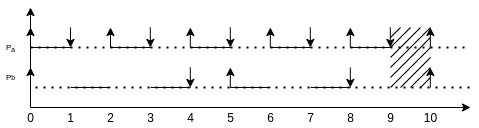
\includegraphics[width=300px]{images/4_Scheduling/rate_monotonic.png}
\end{figure}
\begin{enumerate}
    \setcounter{enumi}{-1}
    \item entrambi i processi hanno lo start quindi metto in esecuzione $P_a$ perché ha priorità maggiore
    \item il processo $P_a$ finisce e metto in esecuzione $P_b$
    \item arriva una richiesta di $P_a$ quindi eseguo preemption e lo metto in esecuzione
    \item il processo $P_a$ finisce e metto in esecuzione $P_b$
    \item il processo $P_b$ finisce ed arriva una richiesta di $P_a$ quindi lo metto in esecuzione
    \item il processo $P_a$ finisce ed arriva una richiesta di $P_b$ quindi lo metto in esecuzione
    \item arriva una richiesta di $P_a$ quindi eseguo preemption e lo metto in esecuzione
    \item il processo $P_a$ finisce e metto in esecuzione $P_b$
    \item il processo $P_b$ finisce ed arriva una richiesta di $P_a$ quindi lo metto in esecuzione
    \item il processo $P_a$ finisce ma non ci sono altri processi quindi la CPU va in idle
\end{enumerate}
Questi processi sono schedulabili usando rate monotonic!

Si noti che noi conosciamo gli istanti in cui i processi partono perché sono periodici, inoltre la preemption è stata utile per mandare in esecuzione il processo $P_a$ interrompendo $P_b$.

Si ha anche del tempo idle quindi l' efficienza effettiva è del 90\%, questo è positivo in quanto se dovessi introdurre un terzo task avrei del margine con il quale lavorare (per esempio un task con $c_c = 1$ e $t_c = 10$), oppure potrei lavorare alla gestione di eventuali task aperiodici.

Cosa succederebbe se ponessi $P(P_b) > P(P_a)$?
\begin{figure}[H]
    \centering
    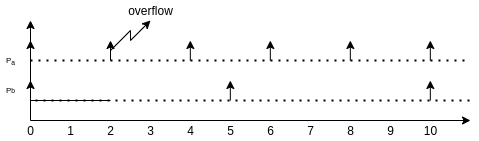
\includegraphics[width=300px]{images/4_Scheduling/rate_monotonic_inverso.png}
\end{figure}
Il sistema non è schedulabile.

Rate monotonic è OTTIMO nella classe degli scheduler a \emph{priorità statica} per \emph{sistemi real time}.
Questo significa che se non riesco a schedularlo con rate monotonic non ce la farò con nessun altro algoritmo a priorità statica. Si potrebbe però usare un algoritmo con priorià dinamica.

\subsubsection{Fattore di utilizzazione}
Possiamo calcolare il numero di volte che il processo $P_i$ esegue nel periodo come: $n_i = \frac{T}{t_i}$, quindi il tempo minimo necessario all' interno del periodo è:
$$ n_1c_1 + n_2c_2 + ... + n_Nc_N = $$
$$ \frac{T}{t_1}c_1 + \frac{T}{t_2}c_2 + ... + \frac{T}{t_N}c_N = T( \sum_{i=1}^{N} \frac{c_i}{t_i} ) \leq T $$
Definiamo quindi \emph{fattore di utilizzazione}: 
$$U \triangleq \sum_{i=1}^{N} \frac{c_i}{t_i} $$
Se so calcolare $U$ posso controllare un primo criterio di schedulabilità, infatti abbiamo che:
$$ U \leq 1 $$
è condizione \emph{necessaria} affinché il sistema sia schedulabile.

Abbiamo poi una condizione sufficiente:
$$ U \leq N \cdot (2^{\frac{1}{N}} - 1) $$
che per $N \xrightarrow{} \infty$ si ha 0.7 quindi se ho almeno il 30\% di CPU libera il sistema è sicuramente schedulabile!

\subsubsection{Earliest deadline first}
In maniera dinamica invece possiamo pensare a mandare prima i processi che hanno la deadline più vicina e che quindi sarebbe bene far terminare il prima possibile.

Es:

$P_a$: $t_a = 4$, $c_a = 2$

$P_b$: $t_b = 10$, $c_b = 5$

$ T=mcm(4,10) = 20 $

\begin{figure}[H]
    \centering
    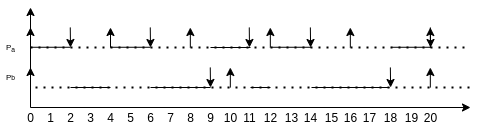
\includegraphics[width=300px]{images/4_Scheduling/edf.png}
\end{figure}
\begin{enumerate}
    \setcounter{enumi}{-1}
    \item entrambi i processi hanno lo start quindi metto in esecuzione $P_a$ perché ha la deadline più vicina

    \setcounter{enumi}{1}
    \item $P_a$ termina e metto in esecuzione $P_b$

    \setcounter{enumi}{3}
    \item arriva una richiesta di $P_a$ quindi eseguo preemption e lo metto in esecuzione perché ha la deadline più vicina

    \setcounter{enumi}{5}
    \item $P_a$ termina e metto in esecuzione $P_b$

    \setcounter{enumi}{7}
    \item arriva una richiesta di $P_a$ ma $P_b$ ha la deadline più vicina quindi continuo con lui
    \item $P_b$ termina e metto in esecuzione $P_a$
    \item arriva una richiesta di $P_b$ ma $P_a$ ha la deadline più vicina quindi continuo con lui
    \item $P_a$ termina e metto in esecuzione $P_b$
    \item arriva una richiesta di $P_a$ quindi eseguo preemption e lo metto in esecuzione perché ha la deadline più vicina

    \setcounter{enumi}{13}
    \item $P_a$ termina e metto in esecuzione $P_b$

    \setcounter{enumi}{15}
    \item arriva una richiesta di $P_a$ ma i due processi hanno la stessa deadline quindi continuo con il processo corrente per avere meno overhead

    \setcounter{enumi}{17}
    \item $P_b$ termina e metto in esecuzione $P_a$

    \setcounter{enumi}{19}
    \item $P_a$ termina ed il periodo ricomincia
\end{enumerate}

NB: questo sistema non sarebbe schedulabile con l' algoritmo rate monotonic ma usando un algoritmo a priorità dinamica ce la facciamo!

NB: abbiamo usato tutto il tempo CPU possibile, quindi $U=1$.

NB: tutto questo è in linea teorica perché stiamo trascurando l' overhead del context switching, ecc.

EDF è l' algoritmo OTTIMO nella classe degli algoritmi di scheduling \emph{dinamici} per i sistemi in tempo reale.


